\section{Validating that the Open-loop System is Unstable}

\begin{questions}
\setcounter{question}{\value{lastquestioncounter}}

\question[2E]
Insert a picture of the time-response of your Segway to the unit-step.

\begin{solution}
   \begin{minipage}[htbp]{\linewidth}
      \centering
      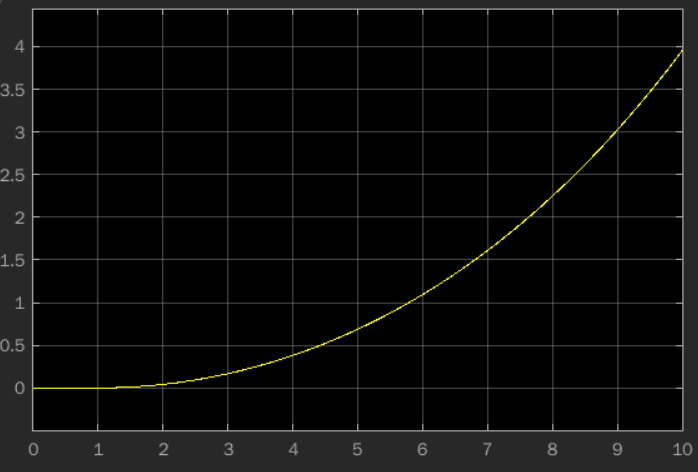
\includegraphics[scale=0.75]{figures/open_loop_time_response.png}
      \captionof{figure}{Time response of the transfer function (\ref{eq:TF_of_Segway_with_values}), $H(s)$, to the unit-step}
   \end{minipage}
\end{solution}

\question[1M]
Comment on whether this time-response indicates that the open-loop system is stable.

\begin{solution}
   The open-loop system is unstable because the response which is y-axis grows faster over time which is x-axis \cite{ref:lecture5}. It can also be deduced from Figure \ref{fig:poles_of_H} because there is a pole in the right-half plane.
\end{solution}

\setcounter{lastquestioncounter}{\value{question}}
\end{questions}
